%Przykładowy plik ułatwiający złożenie projektu dyplomowego inżynierskiego.
%UWAGA: Generowany napis na stronie tytułowej o treści PROJEKT DYPLOMOWY INŻYNIERSKI został zaproponowany przeze mnie i nie jest, póki co, potwierdzony przez władze wydziału. Przed ostatecznym oddaniem tak złożonej pracy należy upewnić się jaka powinna być treść tego napisu. W momencie gdy uzyskam informację na temat treści tego napisu, dokonam niezbędnych zmian w źródłach.

%\documentclass[eng,printmode]{mgr}
\documentclass{mgr}

%opcje klasy dokumentu mgr.cls zostały opisane w dołączonej instrukcji

\usepackage{longtable}

%\input{arduinoLanguage.tex}
%\usepackage[hyphens]{url}
%\usepackage{minted}
\usepackage[newfloat]{minted}
\usepackage{caption}
\usepackage{xcolor} 
\newenvironment{code}{\captionsetup{type=listing}}{}
%\SetupFloatingEnvironment{listing}{name=Source Code}

\definecolor{codeGray}{RGB}{240,240,240} 
\definecolor{codeBlack}{RGB}{0,0,0} 
\definecolor{codeRed}{RGB}{221,0,0} 
\definecolor{codeBlue}{rgb}{0,0,187} 
\definecolor{codeYellow}{RGB}{255,128,0} 
\definecolor{codeGreen}{RGB}{0,119,0}
\usepackage{gensymb}
%poniżej deklaracje użycia pakietów, usunąć to co jest niepotrzebne
%\usepackage{polski} %przydatne podczas składania dokumentów w j. polskim
\usepackage[polish]{babel}%alternatywnie do pakietu polski, wybrać jeden z nich
%\usepackage[cp1250]{inputenc} %kodowanie znaków, zależne od systemu
\usepackage[utf8]{inputenc}
\usepackage[T1]{fontenc} %poprawne składanie polskich czcionek

%pakiety do grafiki
\usepackage{graphicx}
\usepackage{subfigure}
\usepackage{psfrag}

%pakiety dodające dużo dodatkowych poleceń matematycznych
\usepackage{amsmath}
\usepackage{amsfonts}

%pakiety wspomagające i poprawiające składanie tabel
\usepackage{supertabular}
\usepackage{array}
\usepackage{tabularx}
\usepackage{hhline}

%pakiet wypisujący na marginesie etykiety równań i rysunków zdefiniowanych przez \label{}, chcąc wygenerować finalną wersję dokumentu wystarczy usunąć poniższą linię
%\usepackage{showlabels}
%definicje własnych poleceń
\newcommand{\R}{I\!\!R} %symbol liczb rzeczywistych, działa tylko w trybie matematycznym
\newtheorem{theorem}{Twierdzenie}[section] %nowe otoczenie do składania twierdzeń



% moje libki start
\usepackage{tikz-cd}
\usepackage{enumitem}

\usepackage[ruled,vlined]{algorithm2e}
%\usepackage[ruled]{algorithm2e}
\renewcommand{\algorithmcfname}{Algorytm}

\usepackage{float}

%\usepackage[polish]{babel}
%\babelprovide[transforms = oneletter.nobreak]{polish}


%\clubpenalty=10000


%\usepackage[all]{nowidow}

\let\oldref\ref
\renewcommand{\ref}[1]{(\oldref{#1})}

%\usepackage{titlesec}
%\titlespacing*{\section}
%{0pt}{5.5ex plus 1ex minus .2ex}{4.3ex plus .2ex}

\setlength{\parskip}{0cm}
\setlength{\parindent}{1em}
\usepackage[compact]{titlesec}
\titlespacing{\section}{0pt}{4ex}{1ex}
\titlespacing{\subsection}{0pt}{2ex}{0ex}
\titlespacing{\subsubsection}{0pt}{1ex}{0ex}

\usepackage[nodisplayskipstretch]{setspace}
%\setlength{\abovedisplayskip}{0pt} \setlength{\abovedisplayshortskip}{0pt}
%\setlength{\belowdisplayskip}{0pt} \setlength{\belowdisplayshortskip}{0pt}
%\titlespacing{\subsubsection}{0pt}{1ex}{0ex}

\usepackage[bindingoffset=6mm]{geometry}

% moje libki end


%dane do złożenia strony tytułowej
%\title{Tytuł pracy inżynierskiej}
%\engtitle{English title}
\title{Filtry cząsteczkowe i ich zastosowania w~problemach wyznaczania lokalizacji}
\engtitle{Particle filters for selected problems in positioning}
\author{Wojciech Sopot}
\supervisor{dr hab. inż. Paweł Wachel, prof. ucz., W04/K8}
%\guardian{dr hab. inż. Imię Nazwisko Prof. PWr, I-6} %nie używać jeśli opiekun jest tą samą osobą co prowadzący pracę

%\date{2008} %standardowo u dołu strony tytułowej umieszczany jest bieżący rok, to polecenie pozwala wstawić dowolny rok

%poniżej jest lista kierunków i specjalności na wydziale elektroniki, należy wybrać właściwe lub dopisać jeśli nie ma odpowiednich
\field{Automatyka i Robotyka (AIR)}
%\specialisation{Robotyka (ARR)}
%\specialisation{Komputerowe sieci sterowania (ARK)}
\specialisation{Systemy informatyczne w automatyce (ASI)}
%\specialisation{Komputerowe systemy zarządzania \\procesami produkcyjnymi (ARS)}
%\field{Elektronika i telekomunikacja (EIT)}
%\specialisation{Akustyka (ETA)}
%\specialisation{Aparatura elektroniczna (EAE)}
%\specialisation{Elektroniczne i komputerowe \\systemy automatyki (ESA)}
%\specialisation{Zastosowania inżynierii komputerowej \\w technice (EZI)}
%\specialisation{Inżynieria dźwięku (EID)}
%\specialisation{Elektronika stosowana \\i optokomunikacja (TEO)}
%\specialisation{Telekomunikacyjne sieci szerokopasmowe (TSS)}
%\specialisation{Teleinformatyczne sieci mobilne (TSM)}
%\specialisation{Sygnały w telekomunikacji cyfrowej (TSC)}
%\specialisation{Teleinformatyczne systemy rozsiewcze (TSR)}
%\field{Informatyka (INF)}
%\specialisation{Systemy informatyki w medycynie \\i technice (IMT)}
%\specialisation{Inżynieria systemów informatycznych (INS)}
%\specialisation{Inżynieria internetowa (INT)}
%\specialisation{Systemy i sieci komputerowe (ISK)}
%\field{Teleinformatyka (TIN)}
%\specialisation{Teleinformatyka (TIN)}

%tutaj zaczyna się właściwa treść dokumentu
\begin{document}
\bibliographystyle{plabbrv} %tylko gdy używamy BibTeXa, ustawia polski styl bibliografii

\maketitle %polecenie generujące stronę tytułową
%\dedication{6cm}{To jest przykładowa treść opcjonalnej dedykacji, należy ją zmienić lub usunąć w całości polecenie \texttt{$\backslash$dedication}}

\tableofcontents %spis treści
	
\chapter{Wprowadzenie}
W rozdziale przedstawiono cel i zakres pracy oraz podstawowe zadania i problemy wyznaczania lokalizacji. Ponadto opisano ogólną ideę stojącą za filtrami cząsteczkowymi - filtrację bayesowską. 
\section{Zadania i problemy wyznaczania lokalizacji}
Mogłoby się wydawać, iż w dzisiejszych czasach, gdy mamy możliwość korzystania z systemu GPS, nie ma potrzeby zajmować się innymi sposobami wyznaczania lokalizacji. Jednak o ile jest to prawdą w dużej skali, jak np. gdy chce się wyznaczyć adres w mieście pod którym się znajdujemy, to gdy chcemy wyznaczyć swoją lokalizację bardziej dokładnie, np. jak to robią niektóre odkurzacze mobilne, to trzeba wykorzystać do tego dane z innych sensorów, np. lidarów. Czasami można wcale nie mieć możliwości korzystania z systemu GPS, na przykład pod wodą. Innym problemem może być poprawa już znanego przybliżonego położenia. W pracy zostaną przeanalizowane dwa problemy związane z wyznaczaniem lokalizacji:
\begin{itemize}
	\item Określanie położenia samolotu, na podstawie znanej mapy wysokościowej terenu, odczytów z wysokościomierza barometrycznego, oraz, ewentualnie, dodatkowych danych (np. odczytu z kompasu). 
	\item Określanie lokalizacji robota mobilnego, umieszczonego w ograniczonej przestrzeni z przeszkodami (ale na płaskiej powierzchni - mapa jest w dwóch wymiarach).
\end{itemize}
Mimo tego, iż są to jedynie dwa przypadki, w praktyce można je uogólnić na wiele sytuacji. Dla przykładu w \cite{underwater_pf} zajęto się problemem lokalizacji pod wodą, który w praktyce można rozwiązać w ten sam sposób co problem samolotu - mapa wysokości zostaje jedynie zastąpiona przez mapę głębokości.
\section{Cel pracy}
Celem pracy jest rozpoznanie możliwości zastosowania filtrów cząsteczkowych do rozwiązywania problemu lokalizacji oraz samodzielne zaimplementowanie i przebadanie kilku, uznanych arbitralnie przez autora za najciekawsze.
\section{Zakres pracy}
W zakres pracy wchodzi przegląd literatury na temat filtrów cząsteczkowych pod kątem problemów wyznaczania lokalizacji, następnie wybranie kilku rozwiązań oraz ich przebadanie. Aby było to możliwe konieczny jest także przegląd znanych narzędzi programistycznych, które mogą być zastosowane do zaimplementowania algorytmów.

\section{Idea filtracji Bayesowskiej}
Na chwilę obecną, algorytmy oparte o filtrację Bayesowską są szeroko wykorzystywane w automatyce i robotyce. W skrócie, podejście to polega na przeprowadzaniu cykli predykcji i poprawek, na podstawie rozkładu a priori oraz zbieranych w kolejnych iteracjach pomiarów, w celu wyznaczenia rozkładu a posteriori stanu systemu. Ideę tego podejścia widać na rysunku \ref{bayes_fil_idea}. 
\begin{figure}[H]
	\begin{center}
		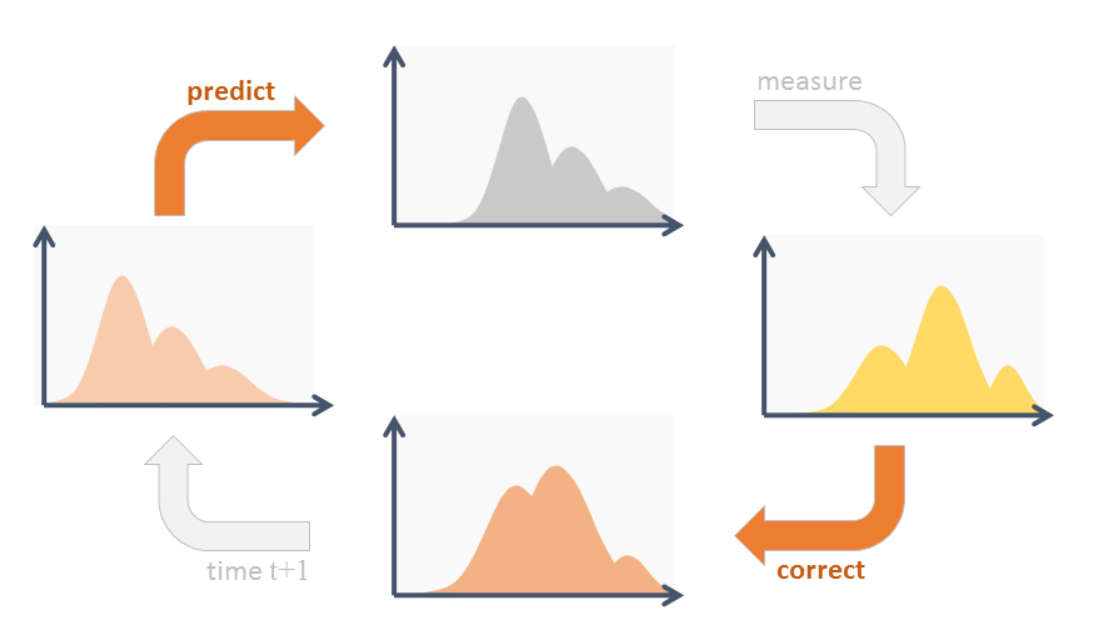
\includegraphics[width=10cm]{./predict_update.png}
		\caption{Idea filtracji Bayesowskiej. Obrazek zaczerpnięto z https://www.codeproject.com/Articles/865934/Object-Tracking-Particle-Filter-with-Ease}
		\label{bayes_fil_idea}
	\end{center}
\end{figure}
Na rysunku \ref{filtr_hier} przedstawiono hierarchię rozwiązać opartych o to podejście. Jak widać jest to bardzo duża rodzina rozwiązań, jednak w pracy zostaną poruszone jedynie metody oparte o filtry cząsteczkowe.
\begin{figure}[H]
	\begin{center}
		\includegraphics[width=10cm]{./nfg001.jpg}
		\caption{Hierarchia filtrów opartych o filtrację Bayesowską. Obrazek zaczerpnięto z \cite{prac_gui}} \label{filtr_hier}
	\end{center}
\end{figure}

\include{filtry_cząsteczkowe}
\include{wybrane_narzędzia_programistyczne}
\chapter{Badania} \label{przeg}
W tym rozdziale opisano przeprowadzone na kodzie badania. Zaczęto od opisania konkretnych problemów którymi się zajmowano, a następnie przeprowadzono badania mające potwierdzić czy algorytmy działają poprawnie. Na koniec przebadano zachowanie zaimplementowane filtry pod różnymi kątami.
\section{Opis poszczególnych problemów}
W badaniach zajęto się dwoma problemami wyznaczania lokalizacji. Pierwszy polega na ustalenie pozycji robota na podstawie pomiaru odległości od ściany, drugi na ustalenie pozycji samolotu na podstawie pomiaru wysokości. W oby przypadkach znano mapę środowiska w którym się znajdowały.
\subsection{Robot w pomieszczeniu} \label{robot_w_pomieszczeniu_desc}
Stan robota w pomieszczeniu opisano czterema liczbami:
\begin{equation*}
	x = \{p_x,p_y,\theta,v\}
\end{equation*}
gdzie $p_x$ i $p_y$ to pozycja robota, $\theta$ jest jego orientacją, natomiast $v$ prędkością. Pomiar odległości od ściany był zawsze wykonywany w kierunku $\theta$, i był miał Gaussowski rozkład. Mapa jest kwadratowym pokojem o wymiarach $1000$ na $1000$ jednostek, wypełnionym kołami o różnych średnicach, oraz ograniczany prostymi. Na rysunku \ref{przykladowa_mapa_pokoju} przedstawiono przykładową mapę.\\
O ile nie będzie napisane inaczej, robot zaczynał na środku mapy, miał prędkość 10 jednostek na iterację, i skręcał w lewo o $0.1rad$ na krok.
\begin{figure}
	\begin{center}
		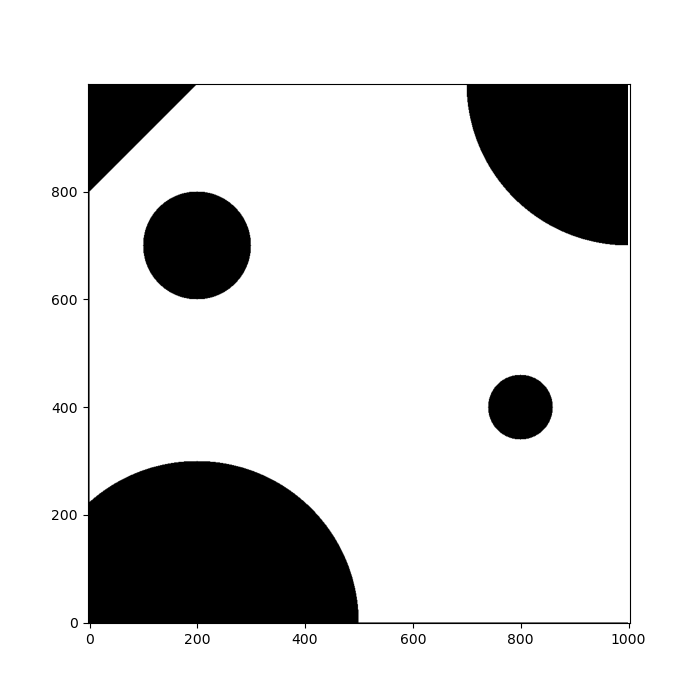
\includegraphics[width=10cm]{./przykladowa_mapa_pokoju.png}
		\caption{Przykładowa mapa pokoju}
		\label{przykladowa_mapa_pokoju}
	\end{center}
\end{figure}
\subsection{Samolot w locie}
Stan samolotu opisano tak samo jak stan robota w rozdziale \ref{robot_w_pomieszczeniu_desc}:
\begin{equation*}
	x = \{p_x,p_y,\theta,v\}
\end{equation*}
Mapa jest natomiast mapą wysokościową, w tym przypadku zdecydowano się na dwa warianty, pierwszy jest mapą fragmentu Wrocławia (przykład widoczny na rysunku \ref{przykladowa_mapa_wroclawia}), natomiast drugą wygenerowano jako szum, którego zmienność można kontrolować (przykład widoczny na rysunku \ref{przykladowa_mapa_szumu}).\\
O ile nie będzie napisane inaczej, samolot w lewym dolnym rogu mapy, miał prędkość 10 jednostek na iterację, i nie zmieniał orientacji $\theta=\frac{\pi}{4}$.
\begin{figure}
	\begin{center}
		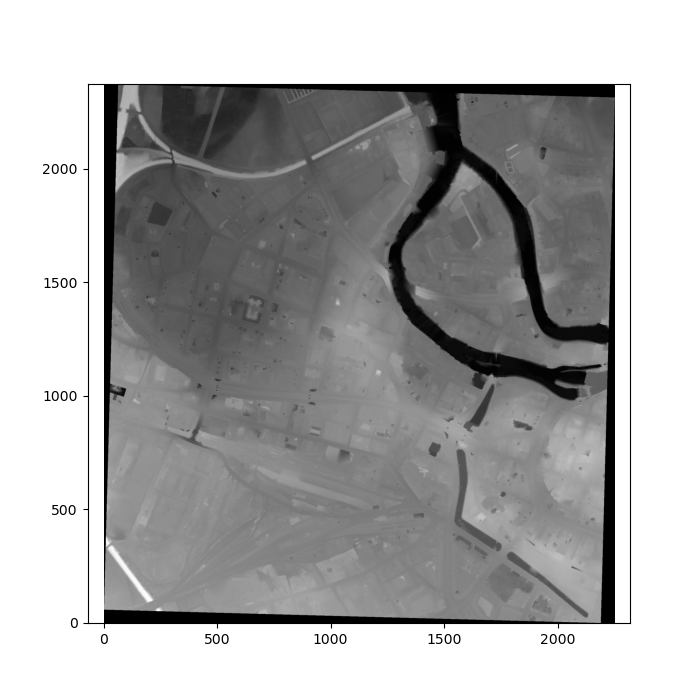
\includegraphics[width=10cm]{./przykladowa_mapa_wroclawia.png}
		\caption{Przykładowa mapa wysokościowa fragmentu Wrocławia}
		\label{przykladowa_mapa_wroclawia}
	\end{center}
\end{figure}
\begin{figure}
\begin{center}
	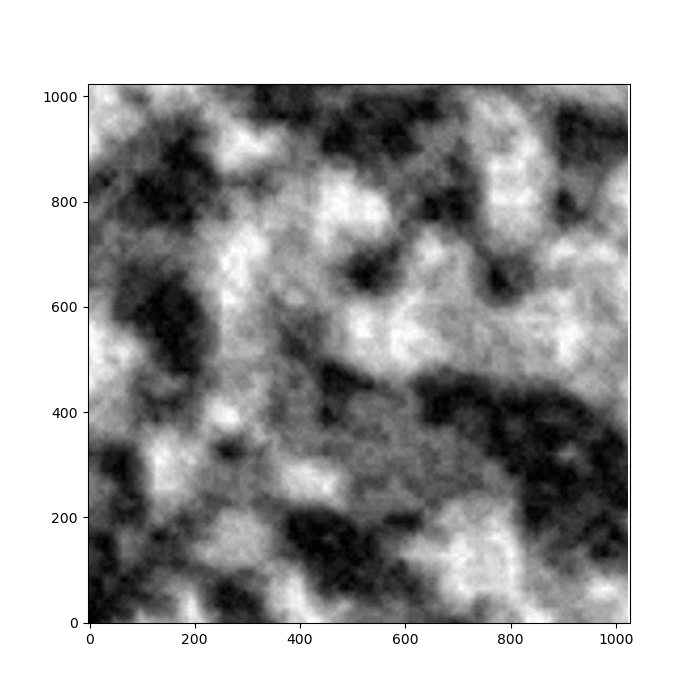
\includegraphics[width=10cm]{./przykladowa_mapa_szumu.png}
	\caption{Przykładowa mapa wysokościowa uzyskana z szumu}
	\label{przykladowa_mapa_szumu}
\end{center}
\end{figure}

\section{Badania poprawności działania}
W tym rozdziale zajęto się badaniami mającymi potwierdzić poprawne działanie zaimplementowanego rozwiązania. Na początku sprawdzono, jak zmiana generatora liczb losowych wpłynęła na wyniki, następnie sprawdzono, jak poradzi sobie algorytm przy braku punktów odniesienia, potem co się dzieje przy braku ewolucji systemu ($v=0$), a na koniec jak filtr radzi sobie z całkowicie losowymi pomiarami. Nie skupiano się no konkretnych wartościach liczbowych, jedynie wizualnie oceniano wyniki.

\subsection{Wpływ generatora}
Przebadano trzy generatory wbudowane w język C++: domyślny linear congruential generator(LCG) \cite{lcg_wiki}, Mersenne Twister \cite{mersenne_wiki} oraz wbudowany niedeterministyczny generator. Populacja cząstek wynosiła $N=1000$. Wyniki rysowano po 1, 11 i 21 iteracjach filtra(nr iteracji oznaczano jako $k$). Wyniki przedstawiono na rysunkach \ref{lcg_example}, \ref{mersenne_example}, \ref{device_example}. Jak widać dla wszystkich generatorów wyniki są niemal takie same, i zbiegają do faktycznego położenia robota. Ponieważ dla każdego generatora uzyskano poprawne wyniki, w dalszych badaniach korzystano z generatora LCG ponieważ jest najprostszy, i, co za tym idzie, najszybszy.

\begin{figure}
	\begin{center}
		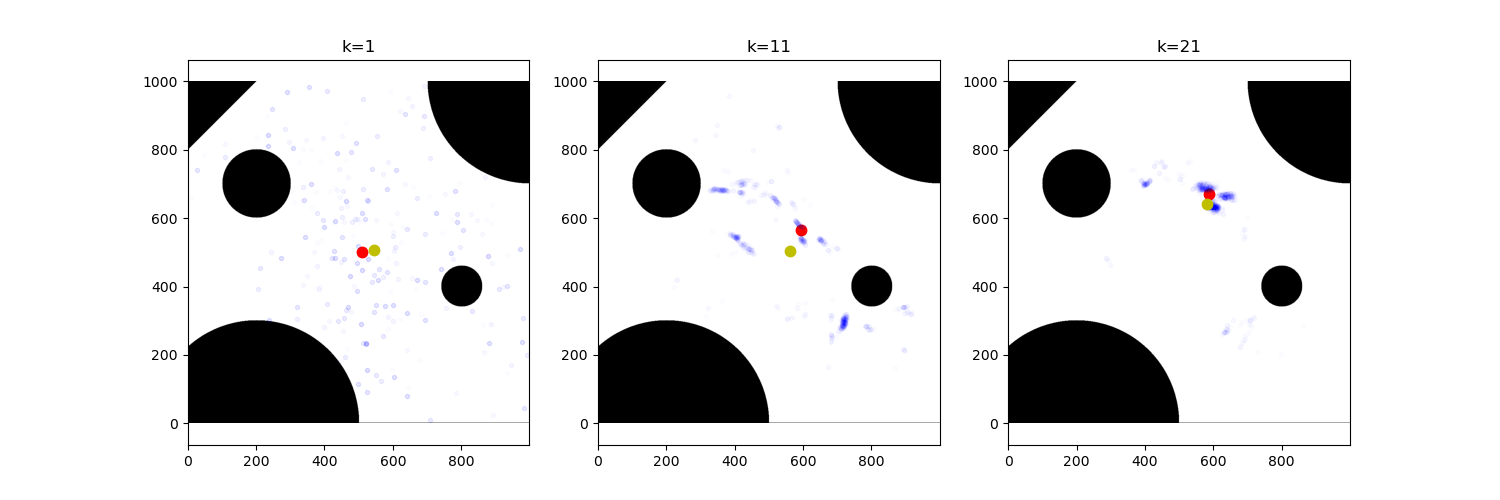
\includegraphics[width=15cm]{./lcg_example.png}
		\caption{Przykładowe wyniki dla generatora LCG}
		\label{lcg_example}
	\end{center}
\end{figure}

\begin{figure}
	\begin{center}
		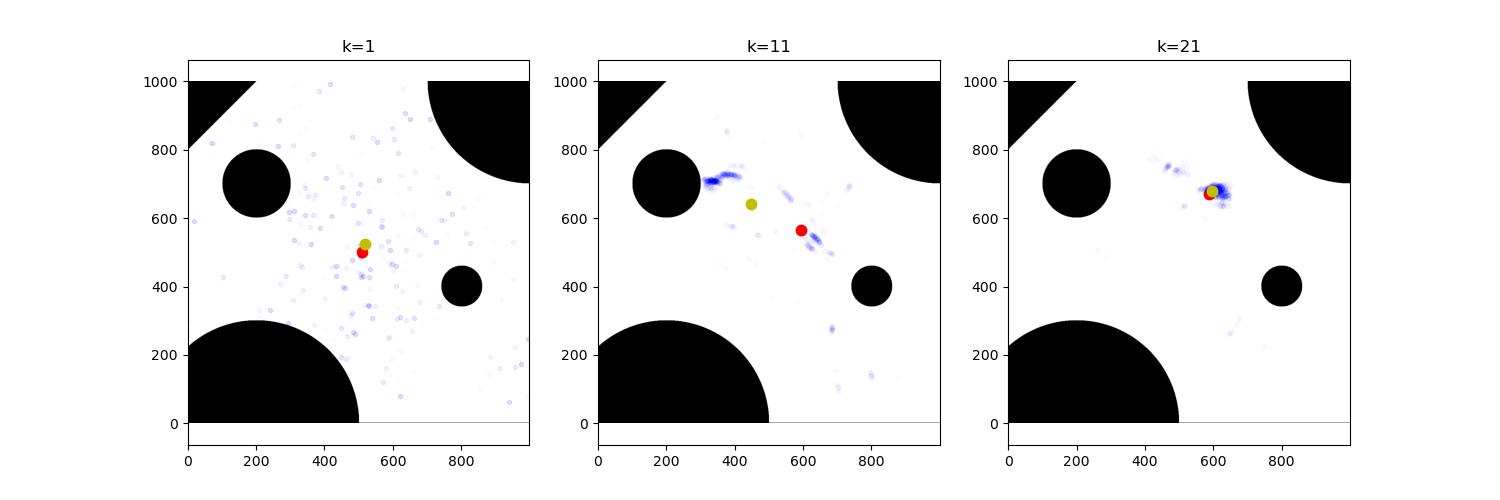
\includegraphics[width=15cm]{./mersenne_example.png}
		\caption{Przykładowe wyniki dla generatora Mersenne Twister}
		\label{mersenne_example}
	\end{center}
\end{figure}

\begin{figure}
\begin{center}
	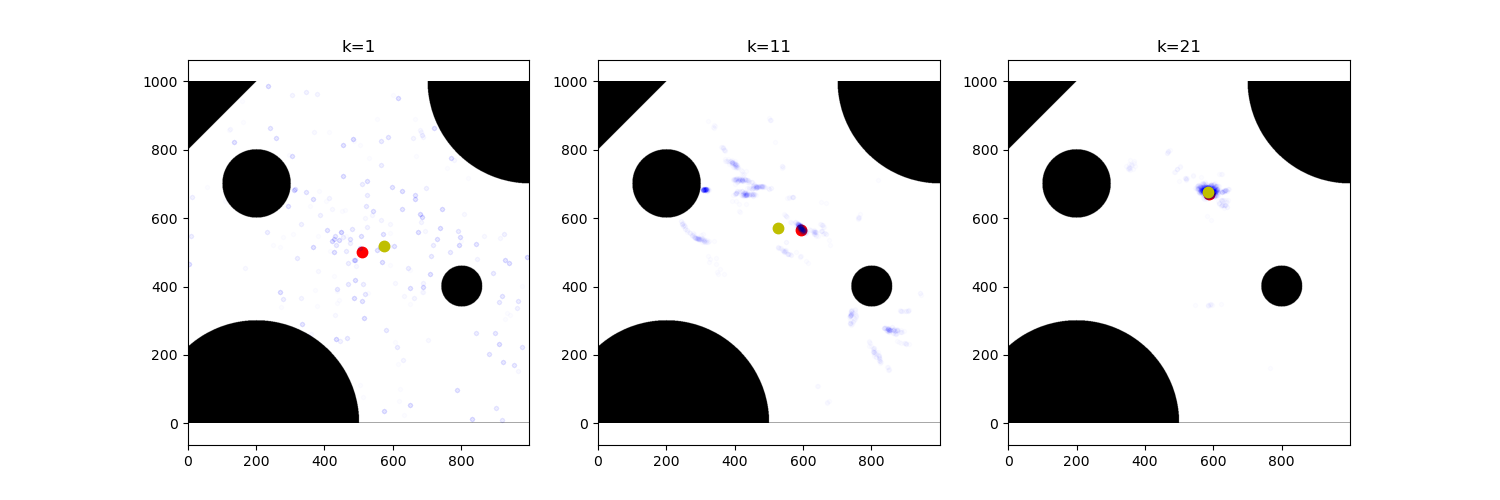
\includegraphics[width=15cm]{./device_example.png}
	\caption{Przykładowe wyniki dla niedeterministycznego generatora}
	\label{device_example}
\end{center}
\end{figure}


\subsection{Niejednoznaczna mapa}
W tym przypadku zbadano jak zachowa się filtr przy braku punktów odniesienia. W kwadratowym pokoju, powinno to spowodować pojawienie się czterech równie prawdopodobnych pozycji. Jak widać przewidywania potwierdziły się na rysunku \ref{no_pivot}. Na rysunku \ref{one_pivot} przedstawiono sytuację, gdy mapa dopuszcza dwie możliwe pozycja. Badania przeprowadzono przy populacji $N=10000$ cząstek.

\begin{figure}
	\begin{center}
		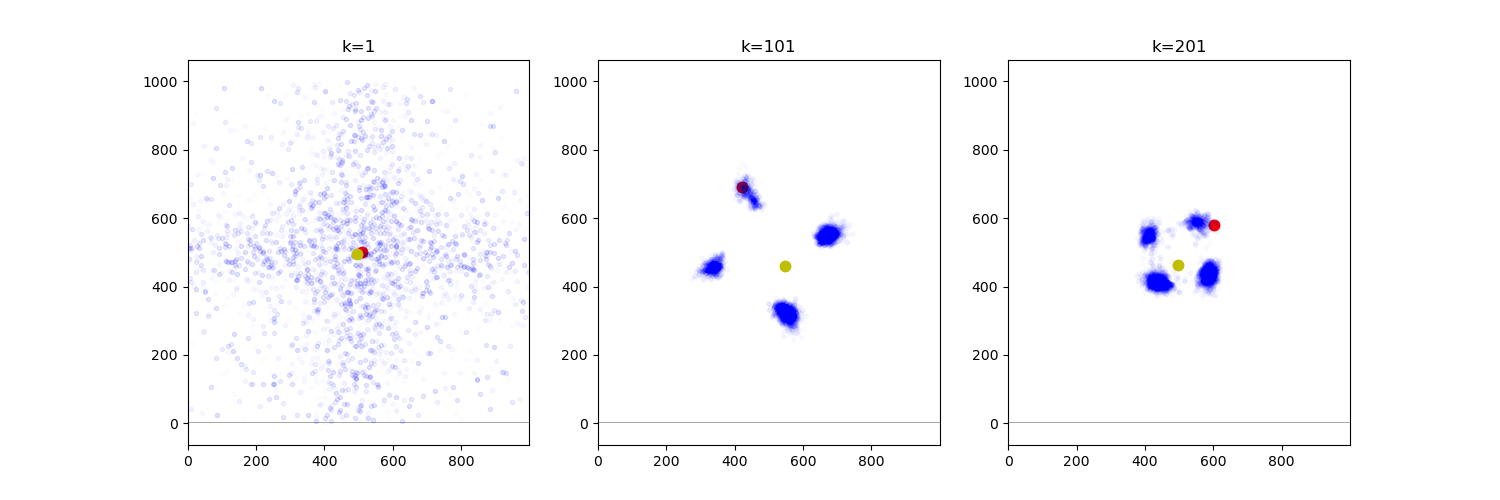
\includegraphics[width=15cm]{./no_pivot.png}
		\caption{Przykładowe wyniki przy braku punktu odniesienia}
		\label{no_pivot}
	\end{center}
\end{figure}

\begin{figure}
	\begin{center}
		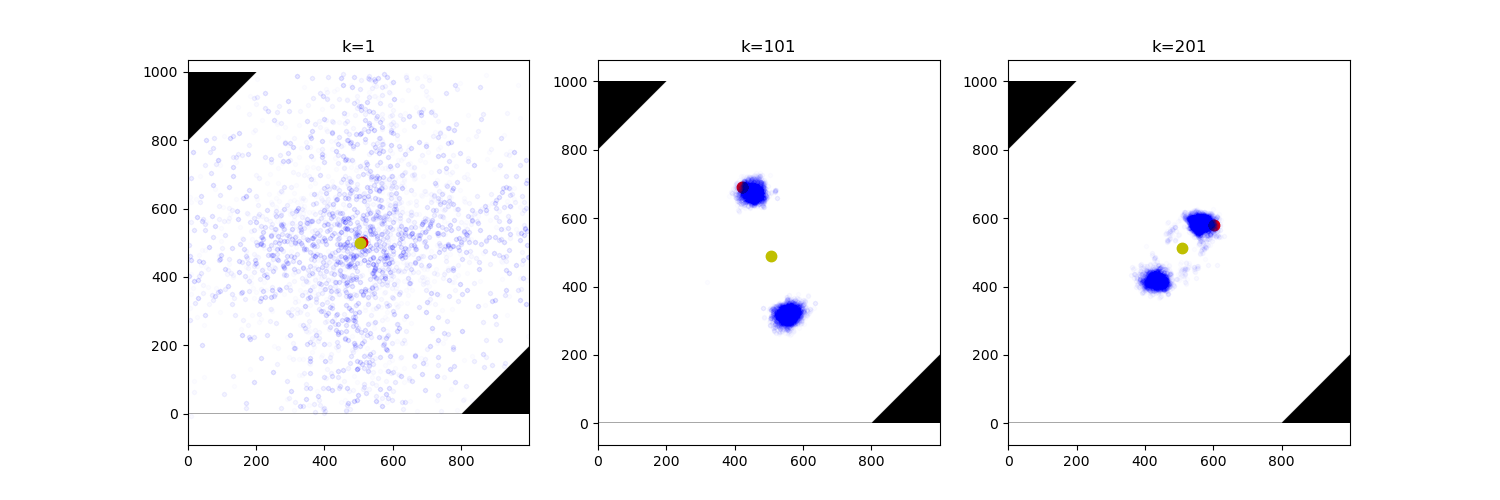
\includegraphics[width=15cm]{./one_pivot.png}
		\caption{Przykładowe wyniki przy dwóch możliwych położeniach}
		\label{one_pivot}
	\end{center}
\end{figure}

\subsection{Brak ewolucji systemu}
Tutaj Zbadano, co się dzieje, gdy system nie ewoluuje. Spodziewano się, pojawią się izohipsy, przynajmniej na początku, nim populacja nie stanie się zbyt zdegenerowana. Badania przeprowadzono dla populacji o rozmiarze $N=100000$. Jak widać na rysunkach \ref{stationary} i \ref{stationary_plane} przewidywania się spełniły, dodatkowo dla rysunku \ref{stationary_plane} dobrze widać pojawianie się degeneracji.

\begin{figure}
	\begin{center}
		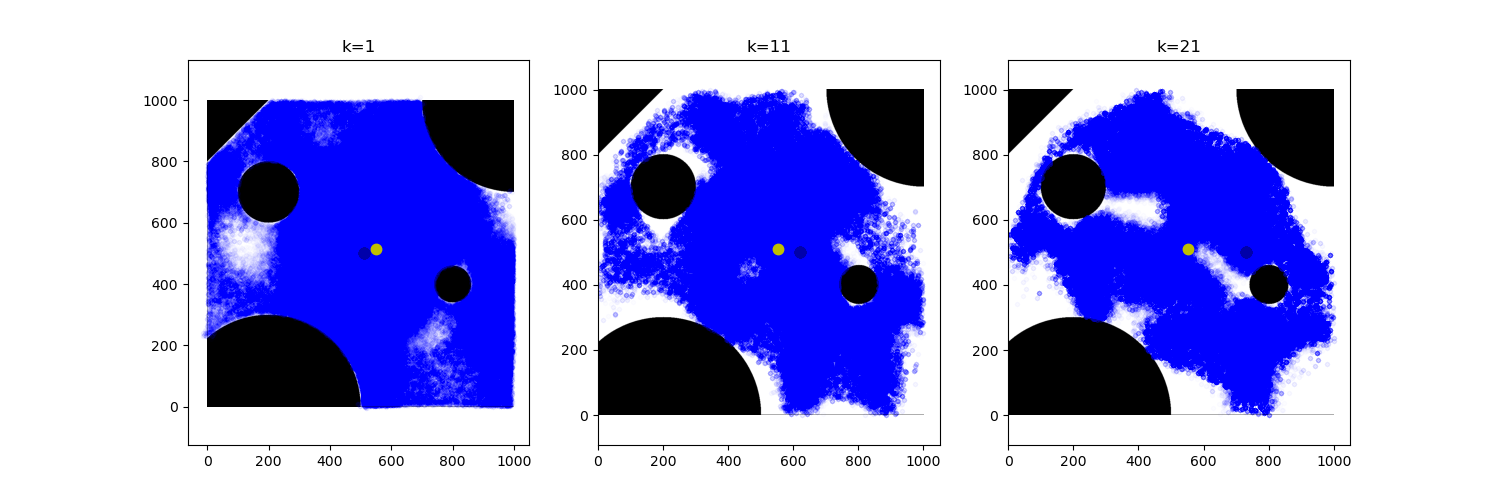
\includegraphics[width=15cm]{./stationary.png}
		\caption{Przykładowe wyniki przy braku ewolucji systemu, dla robota w pokoju}
		\label{stationary}
	\end{center}
\end{figure}

\begin{figure}
\begin{center}
	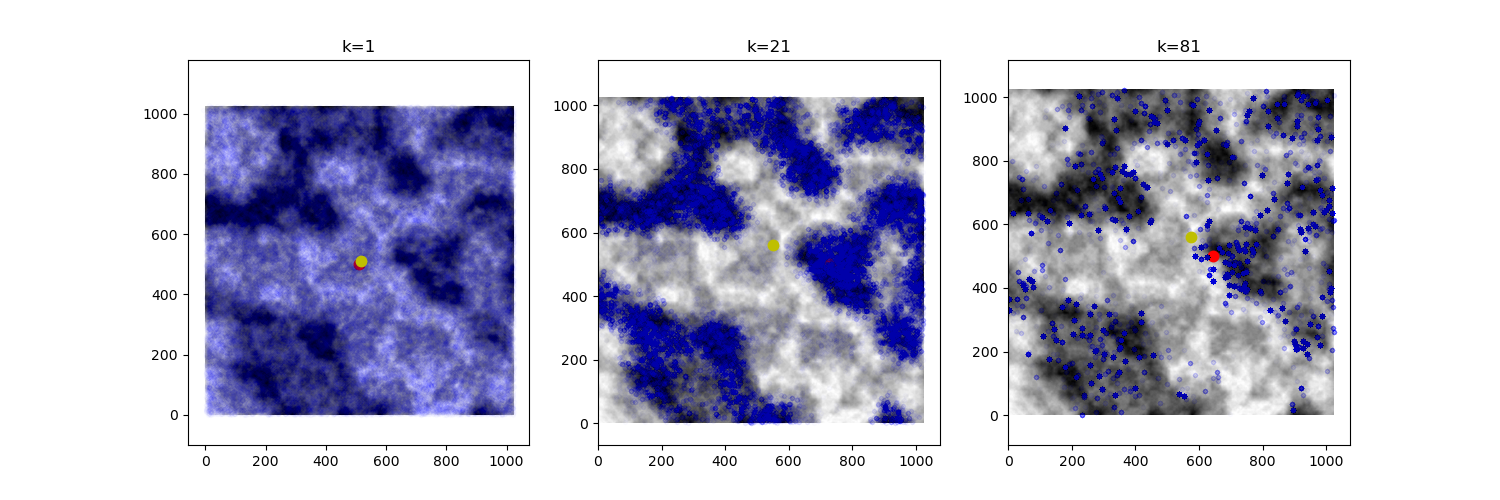
\includegraphics[width=15cm]{./stationary_plane.png}
	\caption{Przykładowe wyniki przy braku ewolucji systemu, dla samolotu}
	\label{stationary_plane}
\end{center}
\end{figure}

\subsection{Pomiary bez związku}
powinien pozostać jednostajny szum

\section{Wpływ sposobu estymowania położenia}
\section{Wpływ funkcji określającej błąd pomiaru}
\section{Wpływ liczby cząstek}
\section{Wpływ metody próbkowania}
\section{Skuteczność w poprawianiu błędnie określonego położenia}
\section{Wpływ szumu}
\section{Wpływ różnorodności terenu}
\section{Rozkład p przy dryfie - chodzi o genetyczne}


\chapter{Wnioski}
\begin{itemize}
	\item 
\end{itemize}
\section{Podsumawanie}
co w kolejnych rozdziałach

\chapter{Kierunki przyszłych badań}
\begin{itemize}
	\item Zrezygnowanie z implementacji C++ na rzecz całkowitego przejścia na Python, z wykorzystaniem na przykład pakietu Numba \cite{numba}. Poza przyspieszeniem porównywalnym z C++, pozwoliło by na przykład na poszerzanie kodu o obliczenia na karcie graficznej. Dzięki temu, można by spróbować rozwiązać problem robota w pokoju, wykorzystując Box Particle Filter.
	\item zamiast avg, np klasteryzacja?
\end{itemize}




%%%%%%%%%%%%%%%%%%%%%%%%%%%%%%%%%%%%%%%%%%%%%%%%%%%%%%%%%%%%%%
%%%%%%%%%%%%%%%%%%%%%%%%%%%%%%%%%%%%%%%%%%%%%%%%%%%%%%%%%%%%%%
%%%%%%%%%%%%%%%%%%%%%%%%%%%%%%%%%%%%%%%%%%%%%%%%%%%%%%%%%%%%%%

%~\cite{WinNT}

\appendix
\chapter{Zawartość załączonej płyty CD}
\begin{itemize}
    \item Praca magisterska - dokument w formacie .pdf
    \item Przygotowane oprogramowanie - pliki w formacie .cpp oraz setup.py
    \item Przygotowane demonstracje - pliki w formacie .py poza setup.py
    \item requirements.txt - opis środowiska Pythonowego
\end{itemize}

\addcontentsline{toc}{chapter}{\bibname} %utworzenie w spisie treści pozycji Literatura
\bibliography{biblio}{} % wstawia bibliografię korzystając z pliku bibliografia.bib - dotyczy BibTeXa, jeżeli nie korzystamy z BibTeXa należy użyć otoczenia thebibliography

%opcjonalnie może się tu pojawić spis rysunków i tabel
 \listoffigures
 %\listoftables

\end{document}
